\documentclass[conference]{IEEEtran}
\IEEEoverridecommandlockouts
\usepackage{cite}
\usepackage{amsmath,amssymb}
\usepackage{booktabs}
\usepackage{graphicx}
\graphicspath{{figures/}}
\usepackage{url}
\usepackage{array}
\usepackage{balance}
\title{Input Novelty and Temporal Performance Degradation in Groundwater Level Prediction: A Study of Training Support and Predictive Stability}
\author{
\IEEEauthorblockN{Amulya P \quad Dhanush R \quad Anagha Kaushik \quad Thrupthi G D}
\IEEEauthorblockA{PES University\\Bengaluru, India}
}
\begin{document}
\maketitle

\begin{abstract}
Groundwater prediction errors may increase when test observations are poorly represented in the training data or when error patterns change over time. We examine these possibilities using 104,781 quarterly groundwater observations from Karnataka, India. A Random Forest was trained on 87,426 observations from 1996--2017 and evaluated on 14,863 observations from 2018--2020. The model achieved an MAE of 1.990 m, compared with 2.601 m for a persistence baseline. Novelty was measured by the mean distance to five nearest training observations in standardised seven-feature space. MAE increased from 1.815 m for well-represented inputs to 3.349 m for very-low-support inputs. Environmental and combined novelty showed increasing error across quartiles, whereas geographic novelty was nearly flat and rainfall-only novelty was non-monotonic. Temporal analyses also found higher errors over the test period: a familiar-input paired comparison across 1,516 wells showed a 0.422 m increase from 2018 to 2020, and a within-well matched-input analysis found a 0.506 m increase across 2,077 pairs. A repeated removal experiment found a small increase in MAE after removing the top 1\% most novel training observations, but its interval reflects variation across model seeds rather than test-well sampling. These results associate prediction degradation with both feature-space support and temporal changes; they do not establish physical causation. Rainfall source and temporal aggregation remain incompletely documented.
\end{abstract}

\begin{IEEEkeywords}
groundwater level prediction, Random Forest, input novelty, distribution shift, temporal stability, rainfall
\end{IEEEkeywords}

\section{Introduction}
Groundwater supports drinking-water supply and irrigation, but its levels vary with recharge, extraction and local hydrogeology \cite{famiglietti,rodell}. Machine-learning models can provide useful groundwater-level estimates, although reported aggregate metrics do not show whether errors are concentrated in unfamiliar input conditions or change during deployment \cite{rajaee,wunsch,sahoo}.

Two explanations are relevant. Input extrapolation occurs when a test observation lies far from the training feature distribution \cite{datasetshift}. Predictive relationship instability is a possible change over time in the association between predictors and the target, often discussed as concept drift \cite{gama}. These mechanisms are related but not interchangeable: a change in the input distribution does not by itself demonstrate a change in the conditional input--target relationship.

This study asks: when groundwater prediction errors increase under unusual conditions, to what extent are they associated with unfamiliar feature combinations, and do errors also increase over time when input support is restricted or matched?

The study makes three empirical contributions using a Karnataka groundwater dataset:
\begin{itemize}
\item It measures training-referenced novelty in geographic, environmental, combined and rainfall-only feature spaces, and compares prediction errors across support levels.
\item It examines temporal error changes using paired wells, matched inputs and within-well residual regressions.
\item It tests the sensitivity of model performance to removing highly novel training observations, while distinguishing model-seed variation from test-sample uncertainty.
\end{itemize}

\section{Related Work}
Machine-learning approaches for groundwater-level modelling include tree ensembles and neural networks; comparative reviews describe their use across different hydrogeological settings \cite{rajaee,wunsch}. Studies have also applied machine learning to groundwater changes in agricultural regions \cite{sahoo}. Random Forests provide a non-linear ensemble baseline and are used here without claiming that they represent the full range of groundwater forecasting methods \cite{breiman}.

The distinction between changes in input distributions and changes in the input--target relationship is established in the dataset-shift and concept-drift literature \cite{datasetshift,gama}. Our contribution is not a new definition of these phenomena. We apply complementary diagnostics to a single regional groundwater dataset and examine whether error changes persist under within-well and matched-input comparisons.

\section{Dataset and Study Design}
\subsection{Groundwater observations and target}
The groundwater records are attributed in the repository to the Central Ground Water Board (CGWB) and cover Karnataka. The processed dataset contains 104,781 observations. The target is the quarterly manual groundwater level, in metres below ground surface. Wells are identified using station name and coordinates. After constructing the previous-measurement feature and removing rows missing required inputs, 102,289 observations remain.

\subsection{Rainfall features and provenance}
The processed file contains 30-day and 90-day accumulated rainfall features in millimetres, together with grid-cell identifiers, grid-centre coordinates and quality-control flags. In the repository archive examined for this revision, the raw-data directory contains the groundwater CSV but no rainfall NetCDF files; the rainfall source files, download procedure and aggregation code are therefore not available in this archive. The grid spacing and alignment are structurally consistent with the IMD 0.25$^\circ$ daily gridded rainfall product, but this does not establish provenance. The rolling-window endpoints, treatment of missing daily values and inclusion or exclusion of the observation date remain undocumented. Consequently, strict pre-observation availability of the rainfall features cannot be independently established.

\subsection{Predictors and temporal split}
The seven model predictors are latitude, longitude, 30-day rainfall, 90-day rainfall, previous groundwater level from the same well, and sine and cosine encodings of observation month. The previous groundwater level is constructed by sorting each well chronologically and shifting its target by one observation. This defines a rolling one-step-ahead setting in which the previous measurement is assumed to be available at prediction time; it is not a fixed-origin multi-step forecast.

A chronological split uses observations before 1 January 2018 for training and observations on or after that date for testing. This yields 87,426 training observations (15 May 1996--5 November 2017) and 14,863 test observations (5 January 2018--30 November 2020). Repository validation reports no overlapping well--date keys between the two periods.

\subsection{Data quality}
The processed dataset contains 746 rows with missing rainfall values (0.712\%), 57 negative groundwater readings (0.054\%) and 256 readings above 50 m (0.244\%). Eight training observations carry suspicious 30-day rainfall flags and 16 carry suspicious 90-day flags; no such flags occur in the test period. The repository reports that excluding flagged training rows changes test MAE by less than 0.001 m. Extreme groundwater readings were retained rather than altered without source-level evidence.

\section{Methods}
\subsection{Prediction models}
We compare a persistence baseline, which predicts the next groundwater level as the previous measurement for that well, with a Random Forest regressor. The baseline forest uses 300 trees, a minimum leaf size of three and random state 42. The forest is fitted on unscaled predictors; scaling is used only for novelty calculations. Random Forests are implemented using scikit-learn \cite{pedregosa}.

\subsection{Training-referenced input novelty}
For each feature space, a StandardScaler is fitted using training observations only. Novelty is the mean Euclidean distance to the five nearest training observations. Training reference scores exclude each observation's self-match. The 95th and 99th percentiles of the training novelty distribution (0.3501 and 0.5544, respectively) define well-represented, sparse-support and very-low-support groups. The primary score uses all seven predictors. Separate analyses use five environmental predictors (rainfall, previous groundwater level and seasonal terms), two geographic predictors, and the two rainfall predictors alone.

For feature-type comparison, test observations are divided into quartiles of geographic, environmental and combined novelty. This comparison is distinct from the training-percentile grouping above.

\subsection{Temporal comparisons}
We report annual test MAE and conduct paired comparisons between 2018 and 2020. The familiar-input analysis restricts observations to the well-represented group and includes wells observed in both years. A second analysis matches 2018 and 2020 observations within the same well using five non-geographic predictors (30-day rainfall, 90-day rainfall, previous groundwater level and the two seasonal terms), standardised before calculating Euclidean distances. Within each well, the Hungarian algorithm selects a minimum-cost one-to-one assignment without replacement; pairs with distance greater than 1.0 in standardised feature space are discarded. This yields 2,077 pairs across 1,311 wells. Confidence intervals are estimated by resampling wells with replacement.

To examine temporal changes in residual associations, Random Forest residuals are regressed on standardised environmental and seasonal predictors for wells represented in all three test years. Well fixed effects are removed by within-well demeaning. Three specifications are compared: predictors only, predictors plus year indicators, and predictors plus year-by-predictor interactions. This analysis describes residual associations; it does not identify changes in the Random Forest's learned physical response function.

\subsection{Controlled training-data removal}
The repeated-removal script fits full, top-1\%-novelty-removed and matched-control Random Forest models for ten random states (42--51). The top-1\%-novelty-removed model excludes the 1\% of training observations with the highest seven-feature novelty scores. The matched-control model removes the same number of observations, matched by calendar year. All models are evaluated on the same 14,863 test observations.

An important implementation detail affects interpretation: the top 1\% highest-novelty training rows are selected once from the fixed training novelty ranking and are therefore identical across all ten random states. The ten runs vary the Random Forest random state; matched-control samples also vary by seed. The reported bootstrap interval resamples the ten seed-level MAE differences. It measures variation across model seeds, not uncertainty from resampling test wells or from repeated independent selections of the high-novelty training observations.

\subsection{Uncertainty estimation}
For paired well-level comparisons, 2,000 bootstrap resamples of wells are used unless otherwise stated. The corrected unfamiliar--familiar comparison includes only wells with observations in both groups (824 eligible wells). The repeated-removal interval is a separate seed-level bootstrap and must not be interpreted as a well-cluster confidence interval. Bootstrap procedures follow standard resampling principles \cite{efron}.

\section{Experimental Results}
\subsection{Overall prediction performance}
Table~\ref{tab:baseline} shows that the Random Forest reduced test MAE by 23.5\% relative to persistence. This is an overall result and does not imply uniform performance across input conditions.

\begin{table}[t]
\caption{Baseline performance on the held-out test set}
\label{tab:baseline}
\centering
\footnotesize
\begin{tabular}{lrrrr}
\toprule
Model & $N$ & MAE (m) & RMSE (m) & $R^2$\\
\midrule
Persistence & 14,863 & 2.601 & 4.439 & 0.628\\
Random Forest & 14,863 & 1.990 & 3.498 & 0.769\\
\bottomrule
\end{tabular}
\end{table}

\subsection{Error across full-feature novelty groups}
Table~\ref{tab:novelty} reports the primary seven-feature novelty analysis from the single baseline Random Forest (random state 42). Table~\ref{tab:removal}, by contrast, reports group MAE averaged across ten Random Forest seeds. MAE rises from 1.815 m in the well-represented group to 3.349 m in the very-low-support group. The two less-supported groups also have higher RMSE and positive mean prediction bias. The novelty score represents distance in a combined feature space; it is not a direct measure of drought, flood or extreme rainfall.

\begin{table}[t]
\caption{Prediction error by seven-feature training-referenced novelty}
\label{tab:novelty}
\centering
\footnotesize
\begin{tabular}{lrrrr}
\toprule
Group & Obs. & Wells & MAE (m) & RMSE (m)\\
\midrule
Well-represented & 13,082 & 1,768 & 1.815 & 2.929\\
Sparse-support & 1,090 & 674 & 3.227 & 6.012\\
Very-low-support & 691 & 503 & 3.349 & 6.610\\
\bottomrule
\end{tabular}
\end{table}

\subsection{Which features define novelty?}
The quartile analysis shows different patterns by geographic, environmental and combined feature space. The rainfall-only panel in Fig.~\ref{fig:novelty} instead displays the training-support groups; corresponding rainfall-only Q1 and Q4 values are not available in the archived quartile output and are therefore not reported in Table~\ref{tab:types}. Geographic novelty is nearly flat between the lowest and highest quartiles (MAE 1.901 and 1.905 m). Environmental novelty increases from 1.541 to 2.754 m, while combined novelty increases from 1.386 to 2.874 m. In the rainfall-only analysis, MAE is 1.930 m in the well-represented group, 2.274 m in sparse-support and 1.823 m in very-low-support. Thus, rainfall-only novelty is non-monotonic and does not reproduce the full-feature pattern.

\begin{table}[t]
\caption{MAE in the lowest and highest novelty quartiles}
\label{tab:types}
\centering
\footnotesize
\begin{tabular}{lrrr}
\toprule
Feature space & Q1 (m) & Q4 (m) & Change\\
\midrule
Geographic & 1.901 & 1.905 & +0.2\%\\
Environmental & 1.541 & 2.754 & +78.8\%\\
Combined & 1.386 & 2.874 & +107.3\%\\
\bottomrule
\end{tabular}
\end{table}

\begin{figure}[t]
\centering
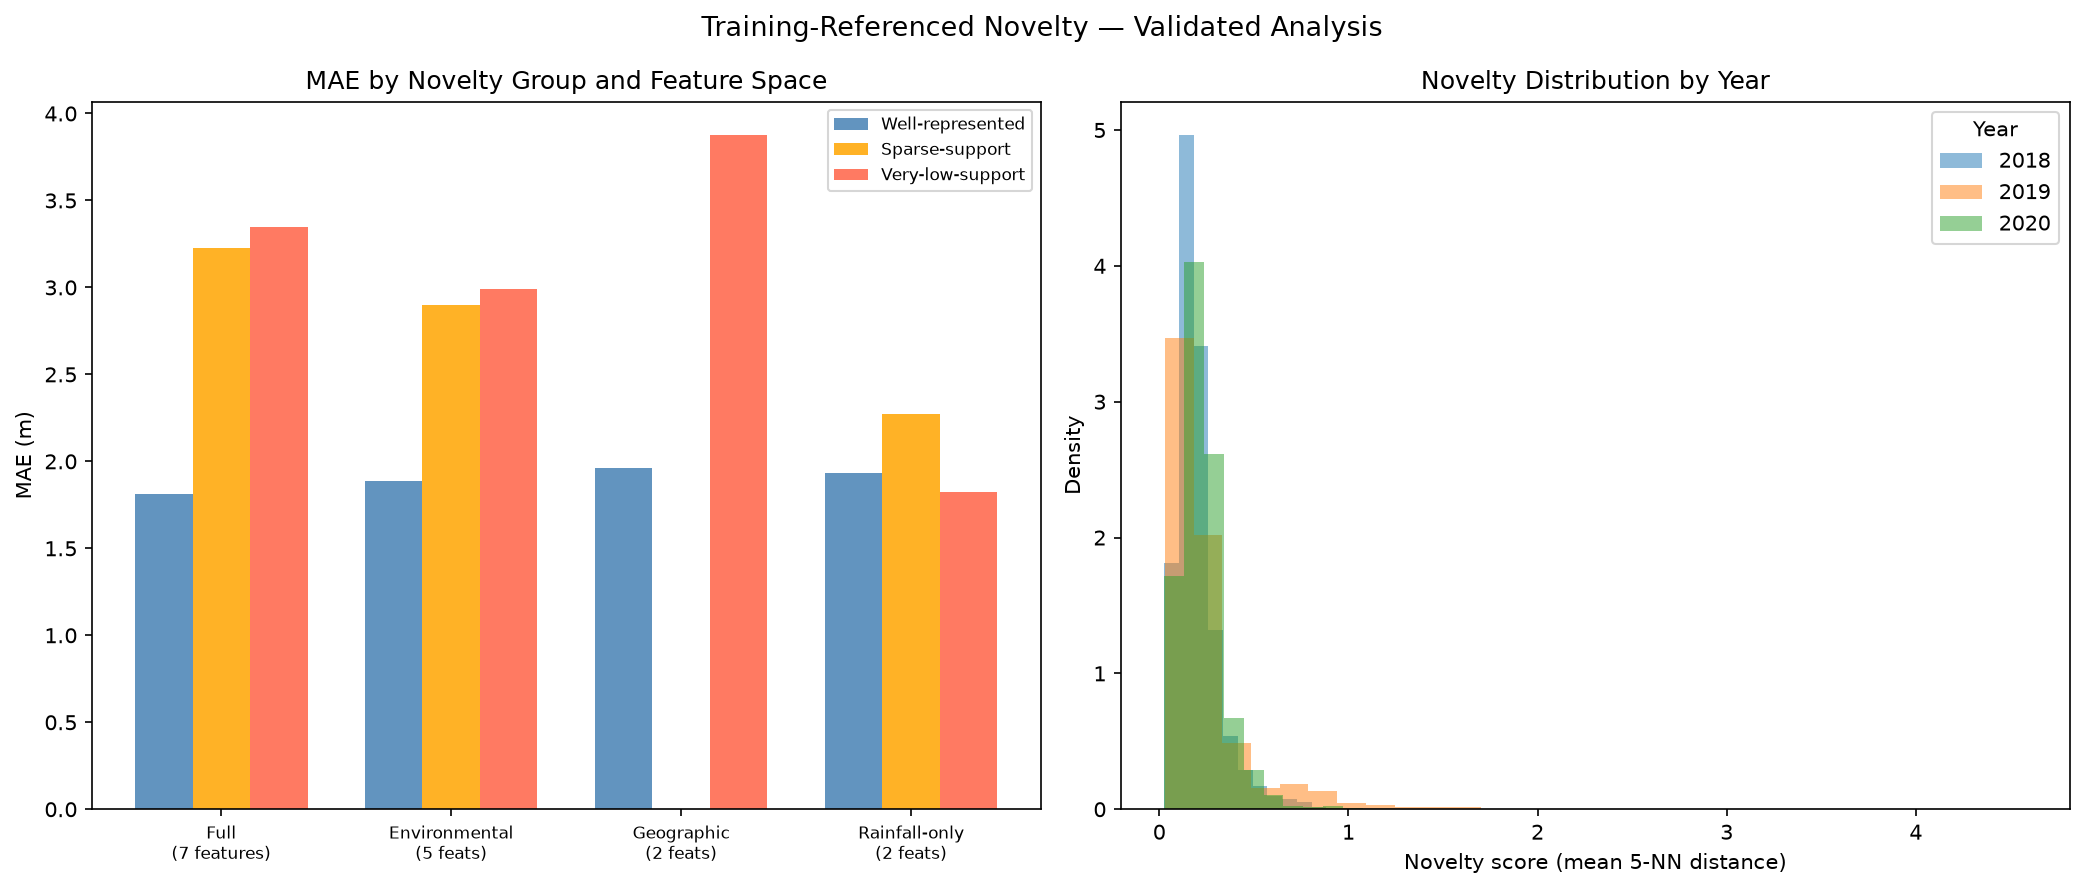
\includegraphics[width=\columnwidth]{figure6_validated_novelty.png}
\caption{MAE across training-referenced novelty groups. Geographic, environmental and combined feature spaces are shown by quartile; the rainfall-only panel uses the separate training-support groups rather than quartiles. Its pattern is non-monotonic.}
\label{fig:novelty}
\end{figure}

\subsection{Rainfall comparisons and within-well confounding}
The unpaired comparison shows lower MAE in the high-rainfall group, but it combines different well populations. In the within-well analysis, 386 wells observed under both conditions have a mean high-rainfall-minus-normal MAE difference of $-0.041$ m (95\% CI: $[-0.169,\,0.080]$ m). The interval includes zero; the unpaired advantage is consistent with between-well differences and does not establish that high rainfall improves prediction.

\subsection{Temporal prediction error}
Across all test observations, MAE increases from 1.804 m in 2018 to 2.291 m in 2020. Among well-represented observations, a paired comparison of 1,516 wells observed in both years gives mean MAE values of 1.709 m and 2.131 m, respectively, a mean increase of 0.422 m (95\% bootstrap CI: [0.303, 0.535] m). The matched-input analysis finds an increase of 0.506 m (95\% CI: [0.410, 0.605] m) across 2,077 matched pairs from 1,311 wells.

\begin{figure}[t]
\centering
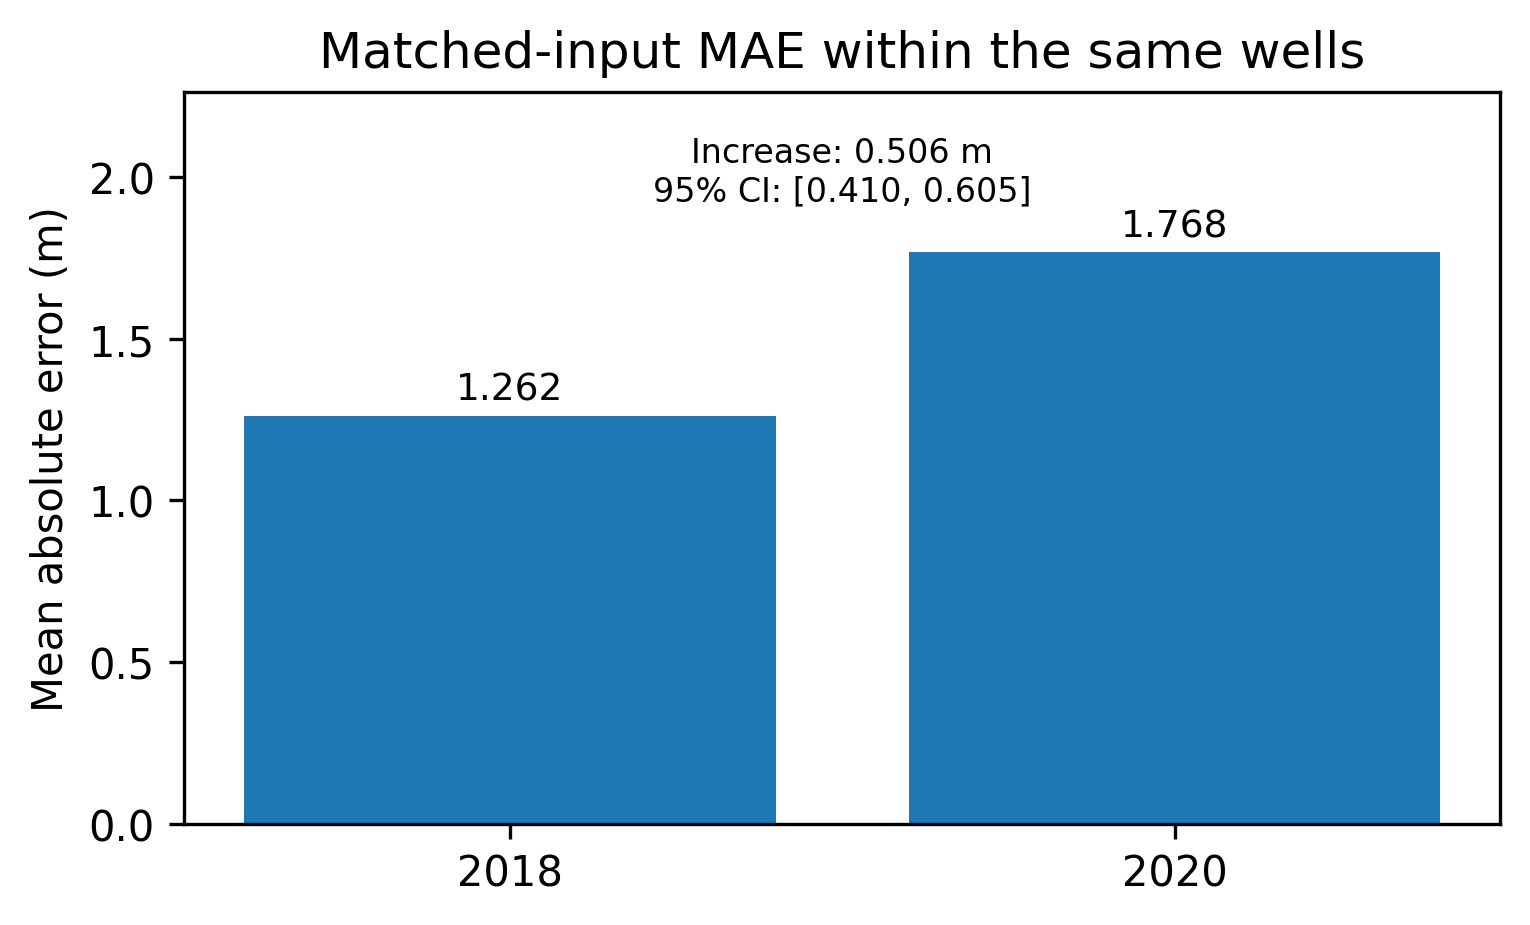
\includegraphics[width=\columnwidth]{figure4_temporal_degradation.png}
\caption{Mean absolute error for the matched-input comparison across 2,077 within-well observation pairs from 2018 and 2020. The increase is 0.506 m (95\% CI: [0.410, 0.605] m).}
\label{fig:temporal}
\end{figure}

\subsection{High-rainfall comparison}
High rainfall is defined using the 95th percentile of 90-day rainfall in the training period (1,219.18 mm). Test observations at or above this threshold form the high-rainfall group; the remaining observations form the normal-rainfall group. For the within-well comparison, we retain wells with at least one observation in each condition (386 wells), calculate each well's mean absolute error separately in the two conditions, and compare the paired high-rainfall-minus-normal difference. The 95\% confidence interval is obtained from 2,000 bootstrap resamples of eligible wells (random seed 42). This is a within-well observational comparison, not a causal estimate.

\subsection{Temporal residual associations}
The within-well residual regression uses 12,142 observations from 1,479 wells represented in all three test years. Adding year indicators changes $R^2$ from 0.2727 to 0.2742; adding year-by-feature interactions increases it to 0.3044. This improvement is consistent with year-dependent residual--input associations. It does not prove that the Random Forest's learned relationship changed, nor does it identify the physical causes of the observed error pattern.

\subsection{Controlled removal of novel training observations}
Across ten model seeds, mean overall MAE was 1.991 m for the full model, 2.006 m after removing the top 1\% most novel training observations, and 1.991 m for the matched-control model. The top-1\%-novelty-removed-minus-full difference was 0.0156 m (95\% seed-level bootstrap CI: [0.0144, 0.0169] m). The mean test novelty distance increased by 8.9\% overall and 25.1\% in the very-low-support group after removal. Table~\ref{tab:removal} reports the mean group MAE across seeds. The largest absolute increase is in the very-low-support group. Because the same top-1\%-novelty training rows were removed for every seed, this experiment does not quantify variability across independent high-novelty-row selections. Its interval captures seed-to-seed model variation only; no test-well bootstrap was performed. The small overall MAE difference should therefore be interpreted as a sensitivity result, not a causal estimate.

\begin{table}[t]
\caption{Mean test MAE across ten model seeds after training-data removal. Table II reports the single baseline model (random state 42).}
\label{tab:removal}
\centering
\footnotesize
\begin{tabular}{lrrr}
\toprule
Test group & Full & Top-1\%-novelty removed & Control\\
\midrule
All & 1.991 & 2.006 & 1.991\\
Well-represented & 1.815 & 1.814 & 1.816\\
Sparse-support & 3.232 & 3.304 & 3.232\\
Very-low-support & 3.350 & 3.598 & 3.349\\
\bottomrule
\end{tabular}
\end{table}

\section{Discussion}
The strongest input-support result is the increase in error across the seven-feature and environmental novelty groups. Geographic distance alone is not informative in the same way, and rainfall-only novelty is non-monotonic. This points to unfamiliar combinations involving rainfall, previous groundwater level and seasonality rather than rainfall extremes alone. Because novelty is a distance-based diagnostic, it should not be interpreted as a physical event label.

The temporal results are also consistent across annual, paired-well and matched-input analyses. The increase among familiar-input wells suggests that changes in the frequency of unfamiliar observations do not fully account for the temporal rise in error. The residual regression adds evidence that residual associations with predictors differ across years. These analyses remain observational: changes in measurement practice, unmeasured pumping and irrigation, geology, land use, and other temporal factors could contribute.

The controlled-removal experiment offers limited additional evidence that removing locally novel training observations can increase test novelty and slightly worsen overall MAE. However, the high-novelty subset was fixed across the ten runs, and the bootstrap reflects model-seed variation only. The result should not be described as evidence of a causal effect of high-novelty training observations.

For deployment, aggregate test metrics should be supplemented with performance stratified by training support and repeated temporal evaluation. The current evidence supports monitoring both input coverage and temporal error, but does not establish a single physical mechanism.

\section{Limitations}
The prediction setup is rolling one-step-ahead and assumes that the previous groundwater measurement is available at prediction time. Feature-space novelty is not equivalent to a physical extreme. Rainfall provenance is unresolved: the repository archive examined here does not include rainfall NetCDF source files or the processing scripts, and the 30-day and 90-day window endpoints and their availability relative to the groundwater observation cannot be verified. The rainfall covariates may therefore carry temporal-alignment uncertainty.

The controlled-removal experiment uses ten model seeds but one fixed set of top-1\%-novelty training observations; its confidence interval does not quantify test-well sampling uncertainty. Matched controls are matched by year, not by well or environmental characteristics. Different analyses also use different eligibility rules and sample sizes. Temporal comparisons cannot fully separate changes in predictive relationships from measurement changes or unobserved drivers such as pumping, irrigation, geology and land use. Finally, the study uses one Karnataka dataset and one chronological split, so generalisation to other regions and aquifer systems is unknown.

\section{Conclusion}
On a held-out Karnataka groundwater dataset, Random Forest errors were higher for observations with low training support and increased between 2018 and 2020, including in familiar-input and matched-input comparisons. Environmental and combined novelty were more informative than geographic distance, while rainfall-only novelty was non-monotonic. Residual regressions showed year-dependent associations but did not establish physical concept drift. The repeated-removal result was small and its uncertainty reflects model seeds, not test-well sampling. Future work should verify rainfall provenance and temporal alignment, include relevant hydrogeological and extraction variables, and test the findings on other regions and forecasting horizons.

\section*{Acknowledgment}
The authors acknowledge the Central Ground Water Board (India) for the groundwater observations used in this study.

\begin{thebibliography}{10}
\bibitem{famiglietti}
J. S. Famiglietti, ``The global groundwater crisis,'' \emph{Nature Climate Change}, vol. 4, no. 11, pp. 945--948, 2014.

\bibitem{rodell}
M. Rodell, I. Velicogna, and J. S. Famiglietti, ``Satellite-based estimates of groundwater depletion in India,'' \emph{Nature}, vol. 460, no. 7258, pp. 999--1002, 2009.

\bibitem{rajaee}
T. Rajaee, H. Ebrahimi, and V. Nourani, ``A review of the artificial intelligence methods in groundwater level modeling,'' \emph{Journal of Hydrology}, vol. 572, pp. 336--351, 2019, doi: 10.1016/j.jhydrol.2018.12.037.

\bibitem{wunsch}
A. Wunsch, T. Liesch, and S. Broda, ``Groundwater level forecasting with artificial neural networks: a comparison of long short-term memory (LSTM), convolutional neural networks (CNNs), and non-linear autoregressive networks with exogenous input (NARX),'' \emph{Hydrology and Earth System Sciences}, vol. 25, pp. 1671--1687, 2021, doi: 10.5194/hess-25-1671-2021.

\bibitem{sahoo}
S. Sahoo, T. A. Russo, J. Elliott, and I. Foster, ``Machine learning algorithms for modeling groundwater level changes in agricultural regions of the US,'' \emph{Water Resources Research}, vol. 53, no. 5, pp. 3878--3895, 2017.

\bibitem{datasetshift}
J. Qui\~nonero-Candela, M. Sugiyama, A. Schwaighofer, and N. D. Lawrence, \emph{Dataset Shift in Machine Learning}. Cambridge, MA, USA: MIT Press, 2009.

\bibitem{gama}
J. Gama, I. Zliobaite, A. Bifet, M. Pechenizkiy, and A. Bouchachia, ``A survey on concept drift adaptation,'' \emph{ACM Computing Surveys}, vol. 46, no. 4, Art. no. 44, 2014, doi: 10.1145/2523813.

\bibitem{breiman}
L. Breiman, ``Random forests,'' \emph{Machine Learning}, vol. 45, no. 1, pp. 5--32, 2001.

\bibitem{pedregosa}
F. Pedregosa \emph{et al.}, ``Scikit-learn: Machine learning in Python,'' \emph{Journal of Machine Learning Research}, vol. 12, pp. 2825--2830, 2011.

\bibitem{efron}
B. Efron and R. J. Tibshirani, \emph{An Introduction to the Bootstrap}. New York, NY, USA: Chapman \& Hall, 1993.
\end{thebibliography}
\balance
\end{document}
